\chapter{Case Study 1: Shut the Box}
\label{cs1}

In this case study, we introduce a game called Shut the Box. We first introduce a new type of model, known as an MDP, allowing for decision making during a game. We then model Shut the Box using an MDP, analyse multiple variants of this game under different strategies, and use this analysis to evaluate the design of Shut the Box.

\section{Shut the Box description}
\label{cs1:stb_description}

Shut the Box is a single player game, where the player aims to cover as many boards as possible through a series of dice rolls. The game starts with a series of \emph{boards}, which are wooden panel on hinges in the physical version, as shown in Figure \ref{cs1:physical_stb}, each numbered sequentially starting from 1, with each board originally uncovered. Each round, the player rolls a set of dice. The player must then cover a set of uncovered boards whose sum is equal to the sum of the dice. For instance, if the player rolls a 1 and a 2, then the player must either cover boards 1 and 2, or cover board 3. When a board is covered, it can no longer be considered when covering future boards. For instance, in the above example, if board 2 has already been covered, the player must cover  board 3, providing that board 3 is still uncovered. The game proceeds in this manner until the player cannot cover a set of uncovered boards which match the values of the dice rolled. A player's \emph{score} for a round of Shut the Box is then defined as the sum of all covered boards when the game ends.

\begin{figure}[h]
    \centering
    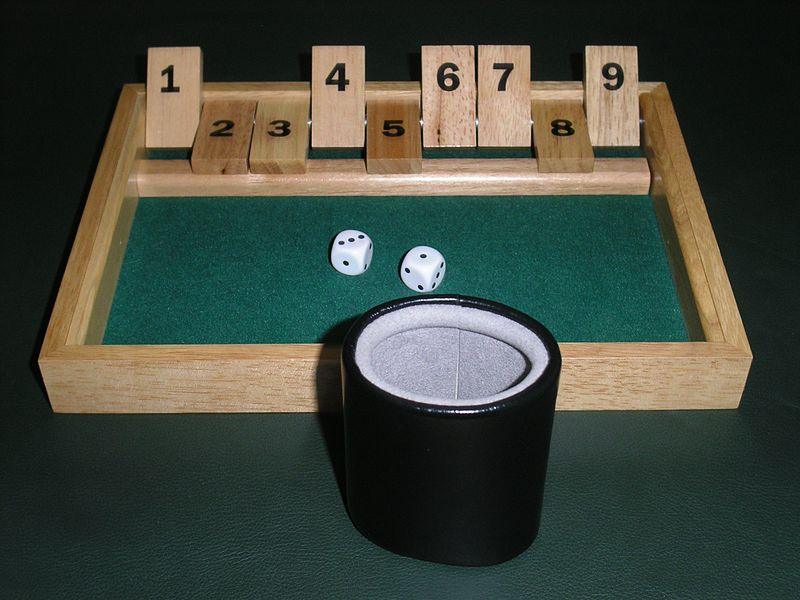
\includegraphics[width=0.7\textwidth]{images/shut_the_box.jpg}
    \caption{A physical version of the 9-board variant of Shut the Box adapted from \cite{wikipedia_deutsch_2006}.}
    \label{cs1:physical_stb}
\end{figure}

Throughout the case study, unless otherwise stated, we consider the variant of Shut the Box where there are 12 boards, and the player rolls two six-sided dice in each round.

When playing Shut the Box, it soon becomes clear that some configurations of boards are highly desirable, while others are more challenging. For instance, consider the situation in Figure~\ref{cs1:cover_choice}, where 4 boards are remaining and suppose the sum of the dice rolled equals 7. As shown in Figure~\ref{cs1:cover_choice}, there are two possible coverings are available. Consider the two possible coverings, we see that leaving boards 1 and 2 uncovered is more valuable than leaving board 3 uncovered - in particular, if a 3 is rolled then every board can be covered in both cases, but if a 2 is rolled then board 2 may be covered in the former case, while no valid covering exists in the latter case. Hence covering boards 3 and 4 leads to a higher expected score at the end of the game than covering boards 1, 2 and 4.

% \begin{figure}[t]
\begin{figure}
    \centering
    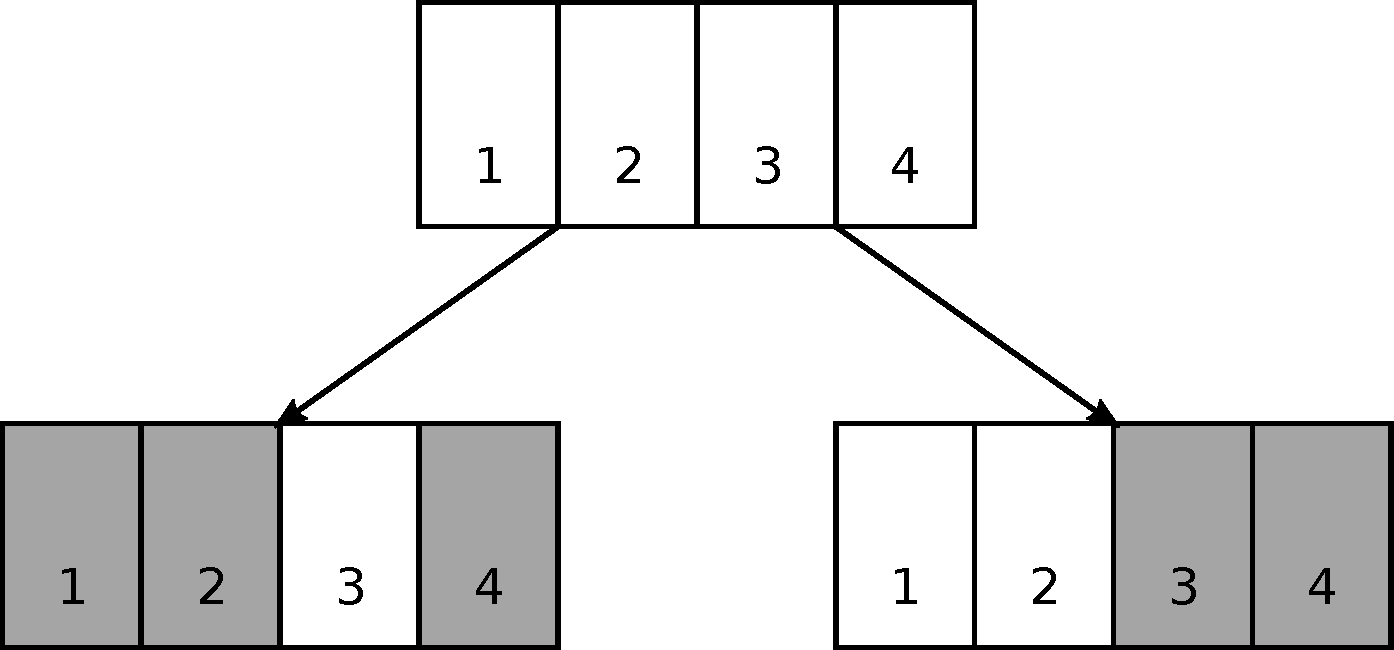
\includegraphics[width=\textwidth]{images/cover_choice.pdf}
    \caption{When boards 1 to 4 are all uncovered, and a 7 is rolled, there are two possible valid coverings - covering boards 1, 2 and 4 (on the left), and covering boards 3 and 4 (on the right).}
    \label{cs1:cover_choice}
\end{figure}

Intuitively, this suggests that lower numbered boards are more valuable later in the game, since they increase the set of possible die rolls that a player can roll without ending the game. From this intuition, we develop two potential strategies for playing Shut the Box. The \emph{high-board strategy} is the strategy where the player always elects to cover the highest number board at each stage, while the \emph{low-board strategy} is the converse, where the player always elects to cover the lowest numbered boards at each stage.

To evaluate the effectiveness of these strategies, model checking is a suitable strategy. Since these strategies are deterministic, we may define DTMCs that model Shut the Box under these two strategies, define the score of the game as a reward structure, and evaluate the expected score when the game terminates. In addition to this analysis, we are also interested in the \emph{optimal} strategy - that is, the strategy which maximises the expected score of Shut the Box. Trying to enumerate and consider every possible strategy would be challenging, both conceptually and computationally. Instead, we consider the nondeterministic variant of the game, where the player makes a nondeterministic choice between all possible coverings after each dice roll, and derive an optimal strategy from here by choosing a series of actions in order to induce an optimal deterministic strategy. In order to achieve this, in the next section we introduce a generalisation of DTMCs which supports nondeterminism.

\section{Background}
\label{cs1:stb_background}

We start by introducing Markov decision processes (MDPs) as described in \cite{forejt_automated_2011}, which are generalisations of DTMCs allowing for actions to be taken at each state, each leading to different probabilistic transitions from that state. We then consider adversaries - resolutions of nondeterministic choice in MDPs - and briefly discuss how optimal adversaries are computed.

\subsection{Markov decision processes}
\label{cs1:mdps}
First, we define an MDP as an extension of a DTMC.

\begin{definition}
\label{cs1:def_mdps}

A Markov decision process (MDP) is a tuple $(S, \bar{s}, A, \delta, L)$, where $S$, $\bar{s}$ and $L$ have the same meanings as in Definition \ref{back:dtmc}. $A$ is the finite set of \emph{actions} on the MDP, while  $\mathbf{\delta} : S \times A \rightarrow Dist(S)$ is the new partial transition probability function, where pairs of states and actions are mapped to probability distributions denoting a transition to another state.

\end{definition}

For example, in a game of Shut the Box, $Act$ is the set of possible subsets of boards that the player can cover (such as the action of covering boards 3 and 5 simultaneously). Hence, $\delta$ maps each state, including the current die value and the current set of uncovered boards, to the set of all possible covering arrangements along with the associated state transition.

A slight extension to paths is required, in order to accommodate that paths also include the actions taken for each transition:

\begin{definition}
\label{cs1:mdp_paths}

An \emph{infinite path} through an MDP is a sequence $s_0 \xrightarrow{a_0} s_1 \xrightarrow{a_1} \dots$ such that $s_i \in S$, $a_i \in A$ and $\delta(s_i,a_i)(s_{i+1}) > 0$ for all $i \in \mathbb{N}$. In other words, each transition under the given action must be possible. A finite path is a truncation of an infinite path.


\end{definition}

Note here that, in general, a state may be associated to more than one action-distribution pair. Indeed, this is where nondeterminism is introduced into the MDP. In order to resolve this nondeterminism, we introduce the concept of adversaries.

\begin{definition}
\label{cs1:adversaries}

Given a \emph{finite} path $\omega = s_0 \xrightarrow{a_0} s_1 \xrightarrow{a_1} \dots \rightarrow{a_{n-1}} s_n$, an adversary is a function $\sigma$ which maps each finite path to an action-distribution pair. Note that, when considering reward-based properties of MDPs, the value of rewards may depend on the actions chosen even if the sequence of states reached remains the same, so our extended definition of paths to include actions is necessary.

\end{definition}

A key remark on this definition is that adversaries make decisions depending on the entire execution history up to and including the state $s_n$, not just the state $s_n$ itself. However, we primarily consider \emph{memoryless adversaries}, where the adversary always picks the same choice in a given state. In particular, this adversary can be viewed as a map from states to actions. Throughout the remainder of the dissertation, we only consider memoryless adversaries unless stated otherwise. We also remark that optimal adversaries for MDPs are non-randomised, so given a particular state the same action is always chosen with probability 1. However this is no longer the case for concurrent games which optimal strategies may require randomisation, which are discussed further in the third case study.

When the behaviour of an MDP is considered under an adversary, the nondeterministic choices are resolved, and a DTMC is obtained. Hence, under a specific adversary, we can apply the model checking techniques introduced in Section \ref{back:prob_mod_check} to evaluate properties of an MDP.

Note that adversaries are often referred to using other names, depending on context, such as schedulers or policies. Throughout this dissertation, by convention we refer to adversaries when discussing the concept over general MDPs, and refer to strategies in the context of a particular game (analogous to a human developing a strategy while playing a game).

We defer discussion on how adversaries are generated until Section \ref{cs1:adversary_gen}. For now, we discuss how optimal values of probabilistic reachability properties are computed, then modify this process in order to provide an adversary which obtains this optimal value.

\subsection{Probabilistic reachability in MDPs}
\label{cs1:prob_reach_mdps}

In a similar manner to Section \ref{back:check-reach}, given an atomic proposition $a$, we define $T$ to be the set of states in some MDP $\mathcal{M}$ where $a$ holds.

Since MDPs allow for nondeterminism, we must consider the minimum and maximum probability of reaching $T$ from each state $s$ of the MDP, over all possible resolutions of nondeterminism. More precisely, for some atomic proposition $a$, and state $s$ (which may not necessarily be an initial state of the associated MDP) we denote these probabilities as $\mathbf{P}^{s}_{min=?} [\mathbf{F} \; a]$ and $\mathbf{P}^{s}_{max=?} [\mathbf{F} \; a]$ respectively. In order to calculate these probabilities, we introduce a method known as \emph{value iteration}, as described in \cite{chatterjee_value_2008}. This method computes a sequence $(x^n_s)_{n \in \mathbb{N}}$, denoting the minimum or maximum probability of reaching $T$ from a given state $s$ within $n$ steps. This sequence then converges to the optimal value, yielding a reasonable approximation of the optimal value for large enough $n$.

First, we perform precomputation of several sets of states, very similarly to precomputation of $S^{yes}$ and $S^{no}$ in Definition \ref{back:S_yes}, where the minimum or maximum reachability probabilities are either 0 or 1. The details of these constructions are omitted and described further in \cite{forejt_automated_2011}. More formally, these precomputed sets are defined as follows.

\begin{definition}
\label{cs1:yes_no}

For a given MDP $\mathcal{M}$, with state space $S$ and atomic proposition $a$:

\begin{itemize}
    \item $S^{yes}_{min}$ is the set of states where $a$ eventually holds with probability 1, regardless of any nondeterministic choice.
    \item $S^{no}_{min}$ is the state of states where $a$ never holds in any subsequent reachable state, for some resolution of nondeterminism.
    \item $S^{yes}_{max}$ is the set of states where $a$ eventually holds with probability 1, for some resolution of nondeterminism.
    \item $S^{no}_{max}$ is the state of states where $a$ never holds in any subsequent reachable state, regardless of any nondeterministic choice.  
\end{itemize}
\end{definition}

We are now ready to define value iteration for calculating the minimum reachability probability for a set of target states $T$, via defining each element in the sequence $(x^n_s)_{n \in \mathbb{N}}$.

\begin{definition}
\label{cs1:value_iteration}

Given an MDP $\mathcal{M}$, with precomputed sets of states as described in Definition \ref{cs1:yes_no}, we have that:

\begin{equation*}
x^n_s = \begin{cases}
        1 & s \in S^{yes}_{min} \\
        0 & s \in S^{no}_{min} \\
        0 & s \notin (S^{yes}_{min} \cup S^{no}_{min}) \; \text{and} \; n=0 \\
        min_{A \in Act} \left\{ \sum_{s' \in S}\delta(s,A)(s') \cdot x^{n-1}_{s'} \right\} & \text{otherwise.} \\
    \end{cases}
\end{equation*}

\end{definition}

Using this method, optimal values can be obtained using an iterative process, and in particular the number of iterations required for a reasonable level of convergence can be determined during the algorithm's execution, such as terminating when the difference between two consecutive terms in the sequence is less than some pre-defined $\epsilon$. However, this specific approach is somewhat flawed, particularly when probabilities are initially small, or the sequence converges slowly. Several pieces of recent work have proposed alternative notions of convergence which address these issues, including the interval iteration algorithm described in \cite{haddad_interval_2018}, which considers upper and lower bounds on value iteration and proceeds until these bounds are sufficiently close together.

We now have a method of approximating $\mathbf{P}^{s}_{min =?} [\mathbf{F} \; a]$ and $\mathbf{P}^{s}_{max =?} [\mathbf{F} \; a]$, which we can then modify to produce not just an approximation of the optimal values themselves, but a method for producing the choices of actions which lead to these optimal values, known as adversary generation, which we discuss in the next section.

\subsection{Adversary generation}
\label{cs1:adversary_gen}

In Definition \ref{cs1:value_iteration}, the inductive step is relatively simple: to find the maximum or minimum probability of reaching a state where $a$ holds within $n$ steps, we consider each possible action, consider each state it can transition to, then consider the probability of reaching a state where $a$ holds from each of these states, and finally choose the action where this value is minimised or maximised.

Hence, to compute the optimal adversary itself, we simply need to select the \emph{action} leading to the optimal value, rather than considering the value itself. Since our adversaries are memoryless and deterministic, and hence defined as a mapping from states to actions, corresponding closely with value iteration. An example of this derivation is given below for calculating a minimum strategy.

\begin{definition}
\label{cs1:min_adv_generation}

Denote $Act(s)$ as the set of actions which are possible within a given state $s$. Then the strategy obtaining the minimum probability of reaching a state where some atomic proposition $a$ holds is given by

\begin{equation*}
    \sigma^{min}(s) = \text{arg min}_{A \in Act(s)} \left\{ \sum_{s' \in S} \delta(s, a)(s') \cdot \mathbf{P}^{s'}_{min =?} [\mathbf{F} \; a]\right\} \, .
\end{equation*}

\end{definition}

A slight modification of this technique is required for the maximum reachability case to prioritise actions which arrive at the set of target states and prevent cycles which never reach the target state. To justify this, consider the following example:

\begin{example}
\label{cs1:bad_valit_example}

Consider the MDP presented in Figure \ref{cs1:bad_mdp_figure}. While in state $s_0$ or $s_1$, the $stay$ action will transition between $s_0$ and $s_1$, while the $exit$ action will transition to the goal state, $s_2$, and consider obtaining $\sigma^{max}(s_0)$ by replacing "min" with "max" in Definition \ref{cs1:min_adv_generation}. The $stay$ and $exit$ actions both have the same maximum value, so either may be selected, and similarly for $\sigma^{max}(s_1)$. But if $\sigma^{max}(s_0) = \sigma^{max}(s_1) = stay$, then the DTMC induced by $\sigma^{max}$ never reaches $s_2$, even though this occurs with probability 1 by selecting the $exit$ action.
\begin{figure*}

\centering
\begin{tikzpicture}[->,>=stealth',shorten >=1pt,auto,node distance=3.5cm,
    scale = 1,transform shape]

\node[state,initial] (s_0) {$s_0$};
\node[state] (s_1) [right of=s_0] {$s_1$};
\node[state,accepting] (s_2) [below of=s_1] {$s_2$};

\path (s_0) edge              node {$stay, 1$} (s_1)
    (s_1) edge              node {$stay, 1$} (s_0)
    (s_0) edge              node {$exit, 1$} (s_2)
    (s_1) edge              node {$exit, 1$} (s_2);

\end{tikzpicture}
\caption{An MDP where the naive approach to adversary generation does not succeed.}
\label{cs1:bad_mdp_figure}
\end{figure*}
\end{example}

%We may still use a similar idea as for minimum adversary generation, but in order to avoid the issue presented in Example \ref{cs1:bad_valit_example}, a slight modification is required to prioritise actions which arrive at the set of target states and prevent cycles which never reach the target state.

Given a specific optimal adversary $\sigma$, computing the reachability probability of an MDP under the adversary is fairly simple, by considering the DTMC induced by $\sigma$ and using the techniques introduced in Section \ref{back:check-reach}. But the converse, that we have shown in this section, is potentially more surprising - given an optimal value for a reachability probability, an adversary can be constructed that obtains this optimal value, during the process of value iteration, with minimal additional computation.

As a final remark, adversary generation for reward-based properties is analogous to adversary generation for reachability properties, using almost identical applications of value iteration and precomputation to compute minimum and maximum expected values until reaching a state where a given atomic proposition holds. For this reason, precise details of constructing these adversaries are omitted.

\section{Results and Analysis (3 pages)}
\label{cs1:stb_results}

In Section \ref{cs1:stb_description}, the high-board and low-board strategies were defined. Our main aim in this study is to analyse these strategies, compare them to the optimal and suboptimal strategies for Shut the Box across different variants, and evaluate the design of Shut the Box based on this information.

\subsection{The one-dice variant}
\label{cs1:stb_one_dice}

Before we examine the standard variant of Shut the Box, we briefly consider the one dice variant with 12 boards, with uniform probability of rolling any number from 1 to 12 inclusive. The probability of obtaining each possible score under each strategy is given in Figure \ref{cs1:stb12_1d12_prob_score}. In particular, we note that the high-board strategy, which we expect to be effective, starts close to the lower bound of probabilities for low scores, then approaches the upper bound for high scores. This indicates an important point about strategies - while the minimum and maximum strategies are represented by continuous lines, they do not represent the same strategy for each score. Rather, they each represent a strategy generated in order to minimise or maximise the probability of obtaining precisely that score. Hence, we would expect an ideal strategy for Shut the Box to have a low probability of obtaining a low score, and a high probability of obtaining a high score.


However, this variant of the game has some flaws. In particular, the probability of achieving a very low score is somewhat high, even for very good strategies. Since each value on a die is equally likely, a succession of low values early on means a low score. In the extreme case, rolling 1 twice in a row means a guaranteed score of 1, regardless of strategy. While this specific example is rare, games should differentiate players based on their strategy, and players can feel frustrated if their strategy makes no difference to the result of the game.

One possible method to alleviate this issue is to alter the probability distribution of a die roll, to reduce the probability of rolling extreme values. This can be simulated by rolling two dice with half as many faces, as a crude approximation of a normal distribution. This is the standard variant of Shut the Box, which is addressed in the next section.

\begin{figure}[h]
    \centering
    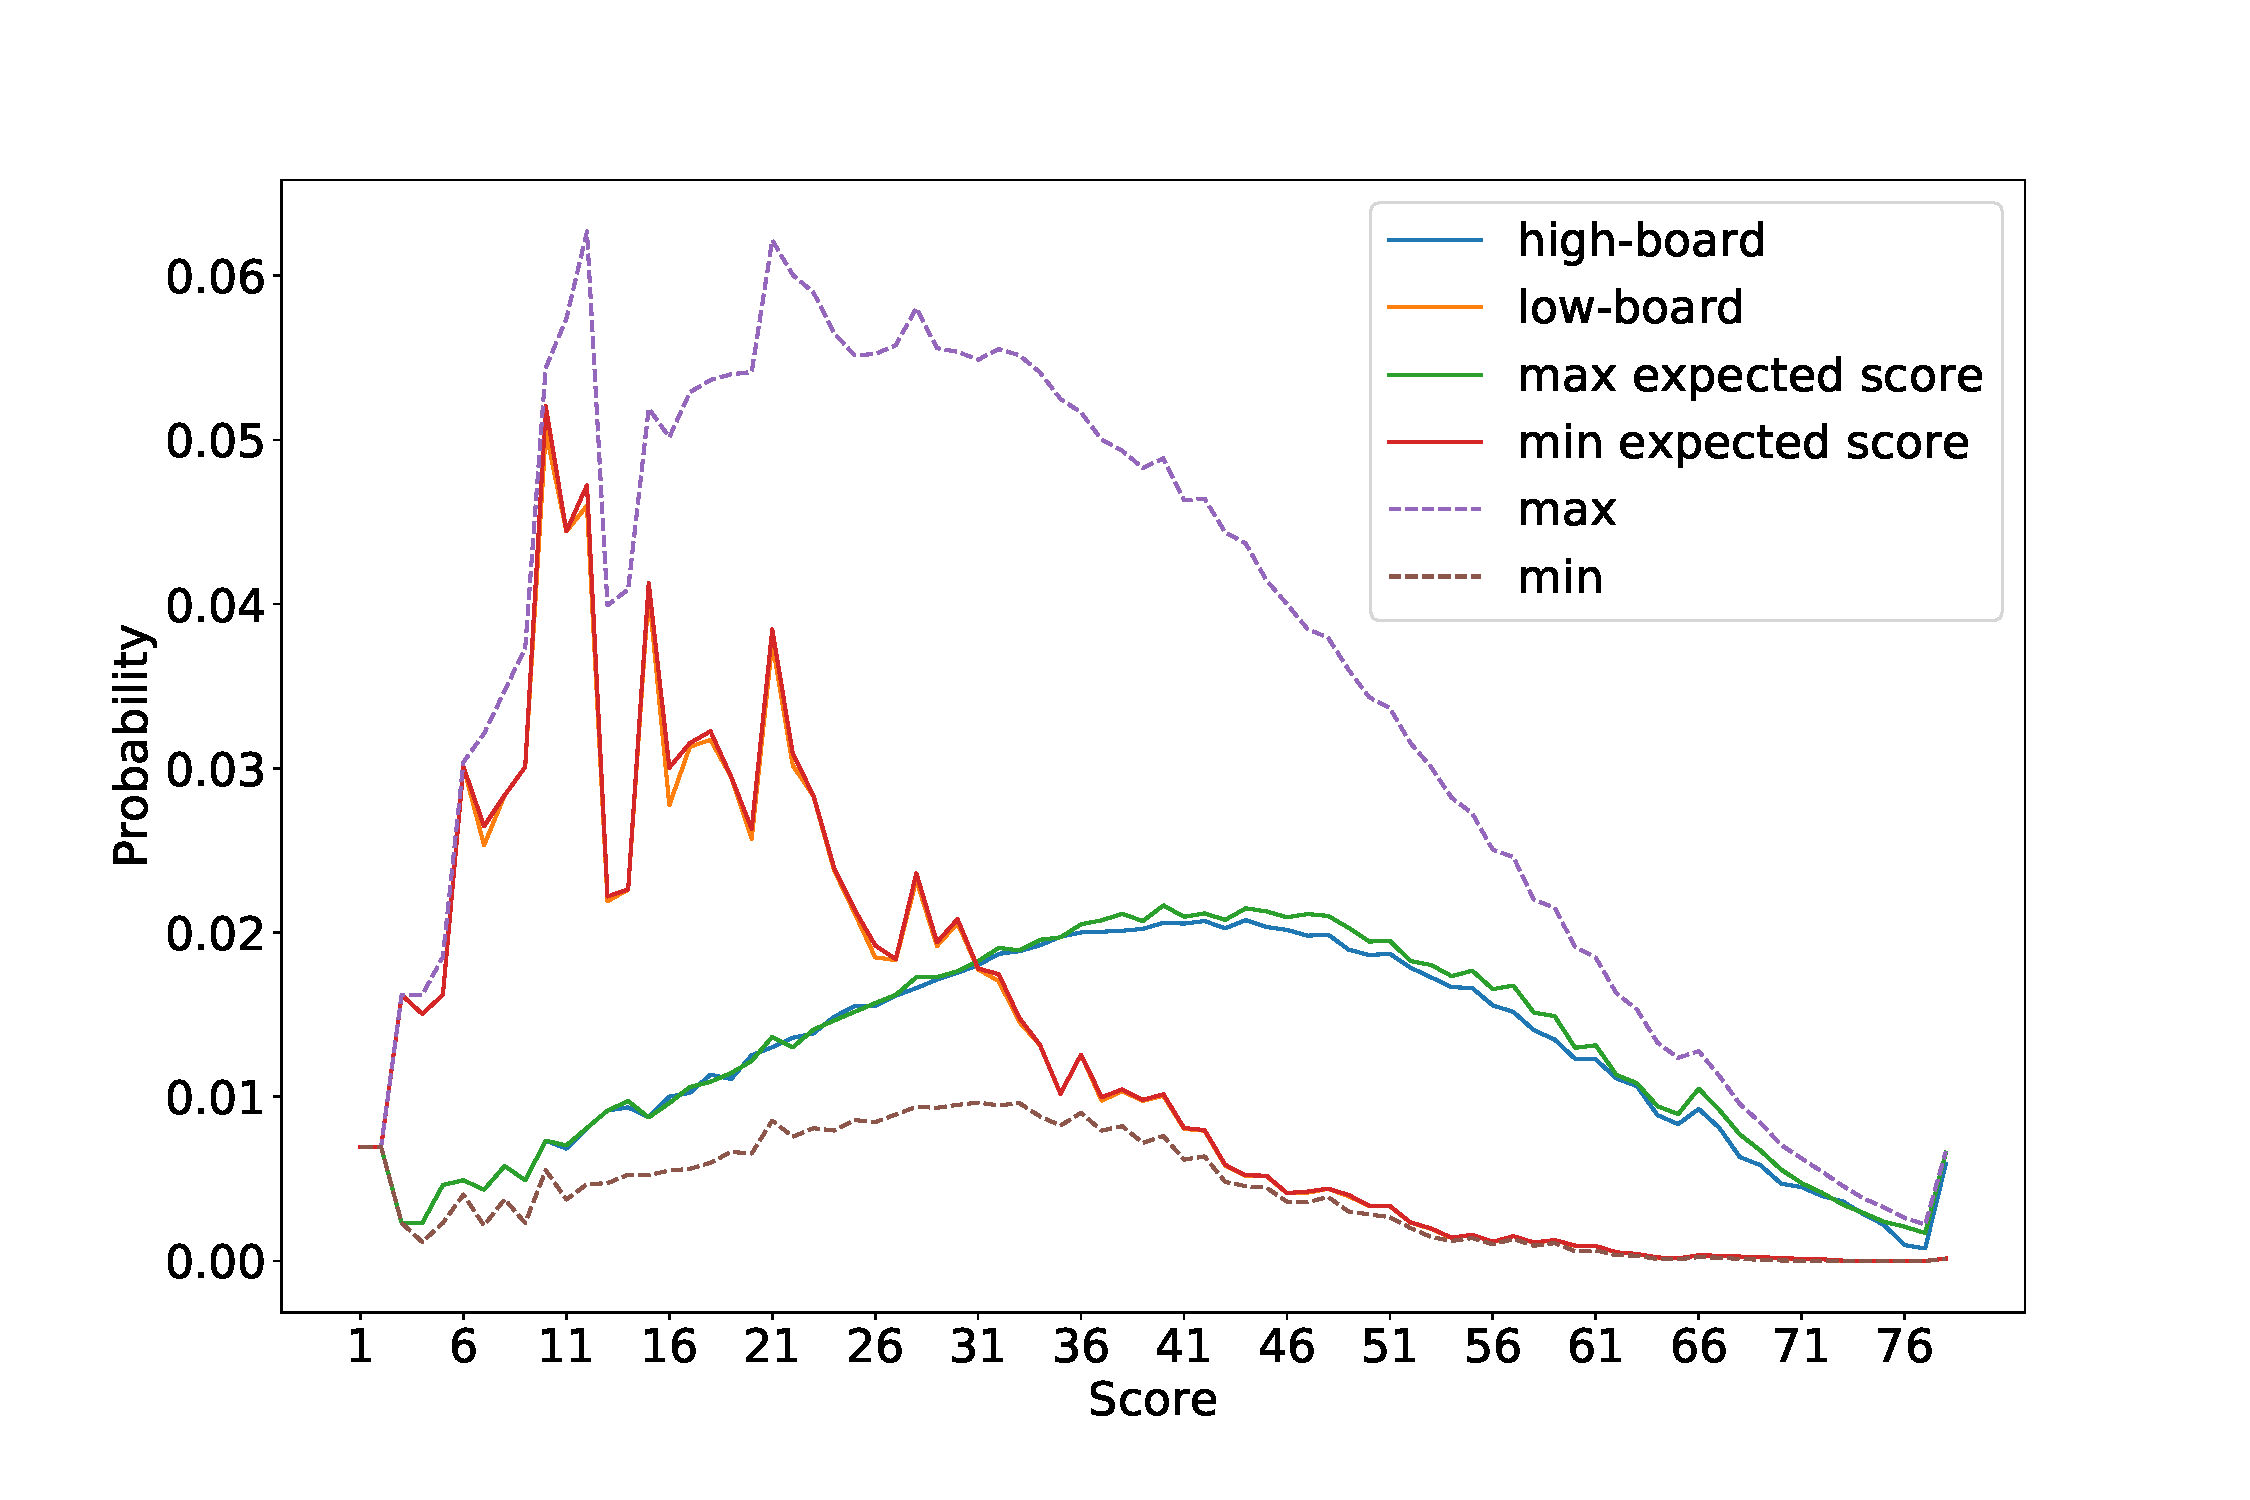
\includegraphics[width=\textwidth]{images/ShutTheBox/stb12_1d12_prob_score.pdf}
    \caption{The probability of obtaining each score in Shut the Box, using one dice, under different strategies.}
\label{cs1:stb12_1d12_prob_score}
\end{figure}

\subsection{The standard variant}
\label{cs1:stb_standard}

\begin{figure}
    \centering
    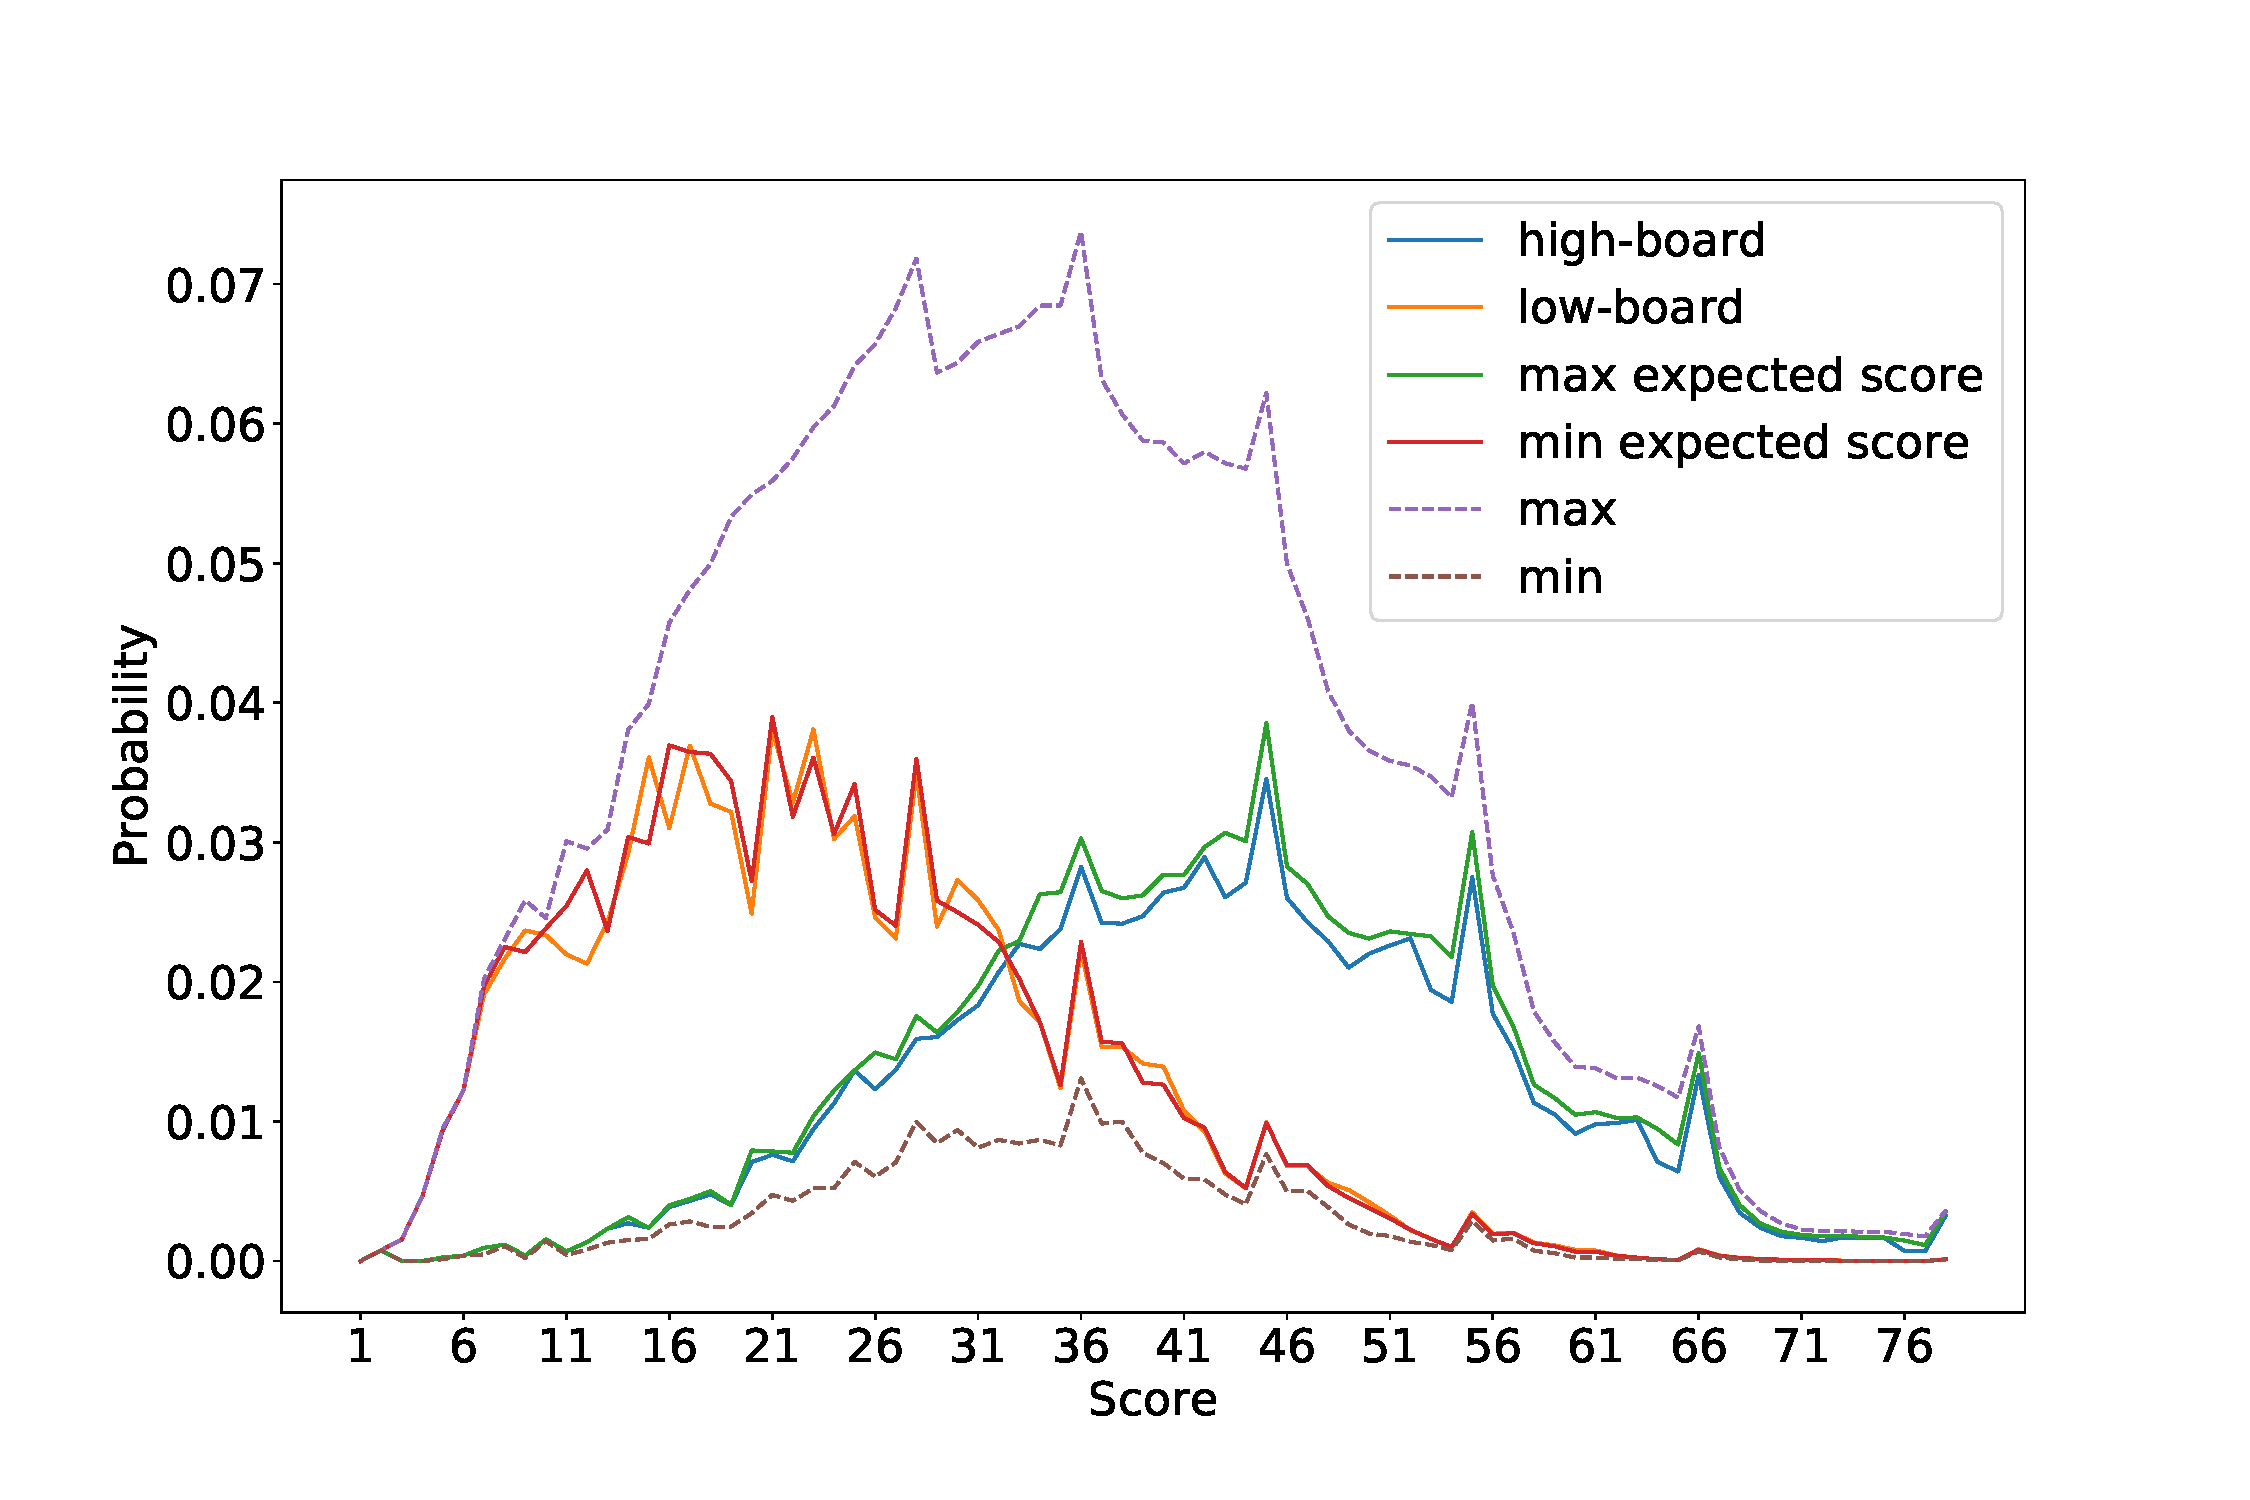
\includegraphics[width=\textwidth]{images/ShutTheBox/stb12_2d6_prob_score.pdf}
    \caption{The probability of obtaining each score in the standard variant of Shut the Box under different strategies.}
\label{cs1:stb12_2d6_prob_score}
\end{figure}

Figure \ref{cs1:stb12_2d6_prob_score} shows the probability of obtaining each possible score in the standard variant of Shut the Box. Immediately we note that the main flaw with the one-die variant of Shut the Box has been mostly resolved, and the probability of obtaining a very low score has been reduced, especially for good strategies.

\begin{table}[h]
    \centering
    \begin{tabular}{@{}ll@{}}
    \toprule
    Strategy used                   & Expected score     \\ \midrule
    \multicolumn{1}{l|}{Minimum expected score}    & 23.9742  \\
    \multicolumn{1}{l|}{Low-board}  & 24.3019 \\
    \multicolumn{1}{l|}{High-board} & 42.8088 \\
    \multicolumn{1}{l|}{Maximum expected score}    & 42.9186
    \end{tabular}
    \caption{The expected score of the standard variant of Shut the Box under different strategies.}
    \label{cs1:exp_value_results}
\end{table}

In particular, the strategies leading to the minimum and maximum expected scores of Shut the Box were generated using PRISM, and the score distributions under these strategies were obtained and visualised. And from figure \ref{cs1:stb12_1d12_prob_score}, the high-board and low-board strategies are very similar to the maximum and minimum expected value strategies respectively. This is further evidenced by Table \ref{cs1:exp_value_results}, showing the overall similarity between the optimal and pre-defined strategies.

In a more abstract sense, the difference between the minimum and maximum strategies represents the impact that strategy can have on the game. For instance, several peaks on strategies occur at triangular numbers, since these present opportunities for bad strategy to significantly impair future rolls. To take a basic example, when no boards are covered, rolling a 10 in the standard variant means that the high-board strategy will cover board 10, while the low-board strategy will cover boards 1, 2, 3 and 4. The former case still allows the game to continue regardless of the value of the next roll, whereas the low-board strategy means that any future rolls between 2 and 4 will always cause the game to end. Therefore, while players can be unlucky regardless of their strategy (for instance, rolling a 2 twice in a row will always lead to the game ending), sound strategy can leave more options open in later rounds.

This initial analysis suggests that the high-board strategy is effective, and even close to optimal for obtaining high scores. We investigate this further in two main directions. We first consider the relative importance of high boards compared to low boards, then generate and compare the optimal strategy with the high board strategy to ascertain their differences.

\subsection{Quantifying the value of high boards}

Intuitively, we expect high boards to be more important than low boards, for several reasons. Firstly, they clearly contribute more to the final score of the game. But more importantly, due to their higher value, there are fewer possible die rolls which can cover high boards, which suggests that an opportunity to cover a high board should be prioritised over covering lower value boards. In essence, this is the key idea behind the high-board strategy. 

To exemplify this, we consider each board in turn, assume that board is covered, and consider the probability of obtaining each score given this covering. The results of this are given in Figure \ref{cs1:stb12_2d6_cond_prob}. In particular, all boards have a positive correlation between the final score and the probability that board is covered, which is unsurprising given that larger scores naturally involve covering more boards, but this correlation is far stronger for higher value boards, suggesting that covering high boards should be prioritised where possible.

% I know this figure is very messy, need to refine this!
\begin{figure}
    \centering
    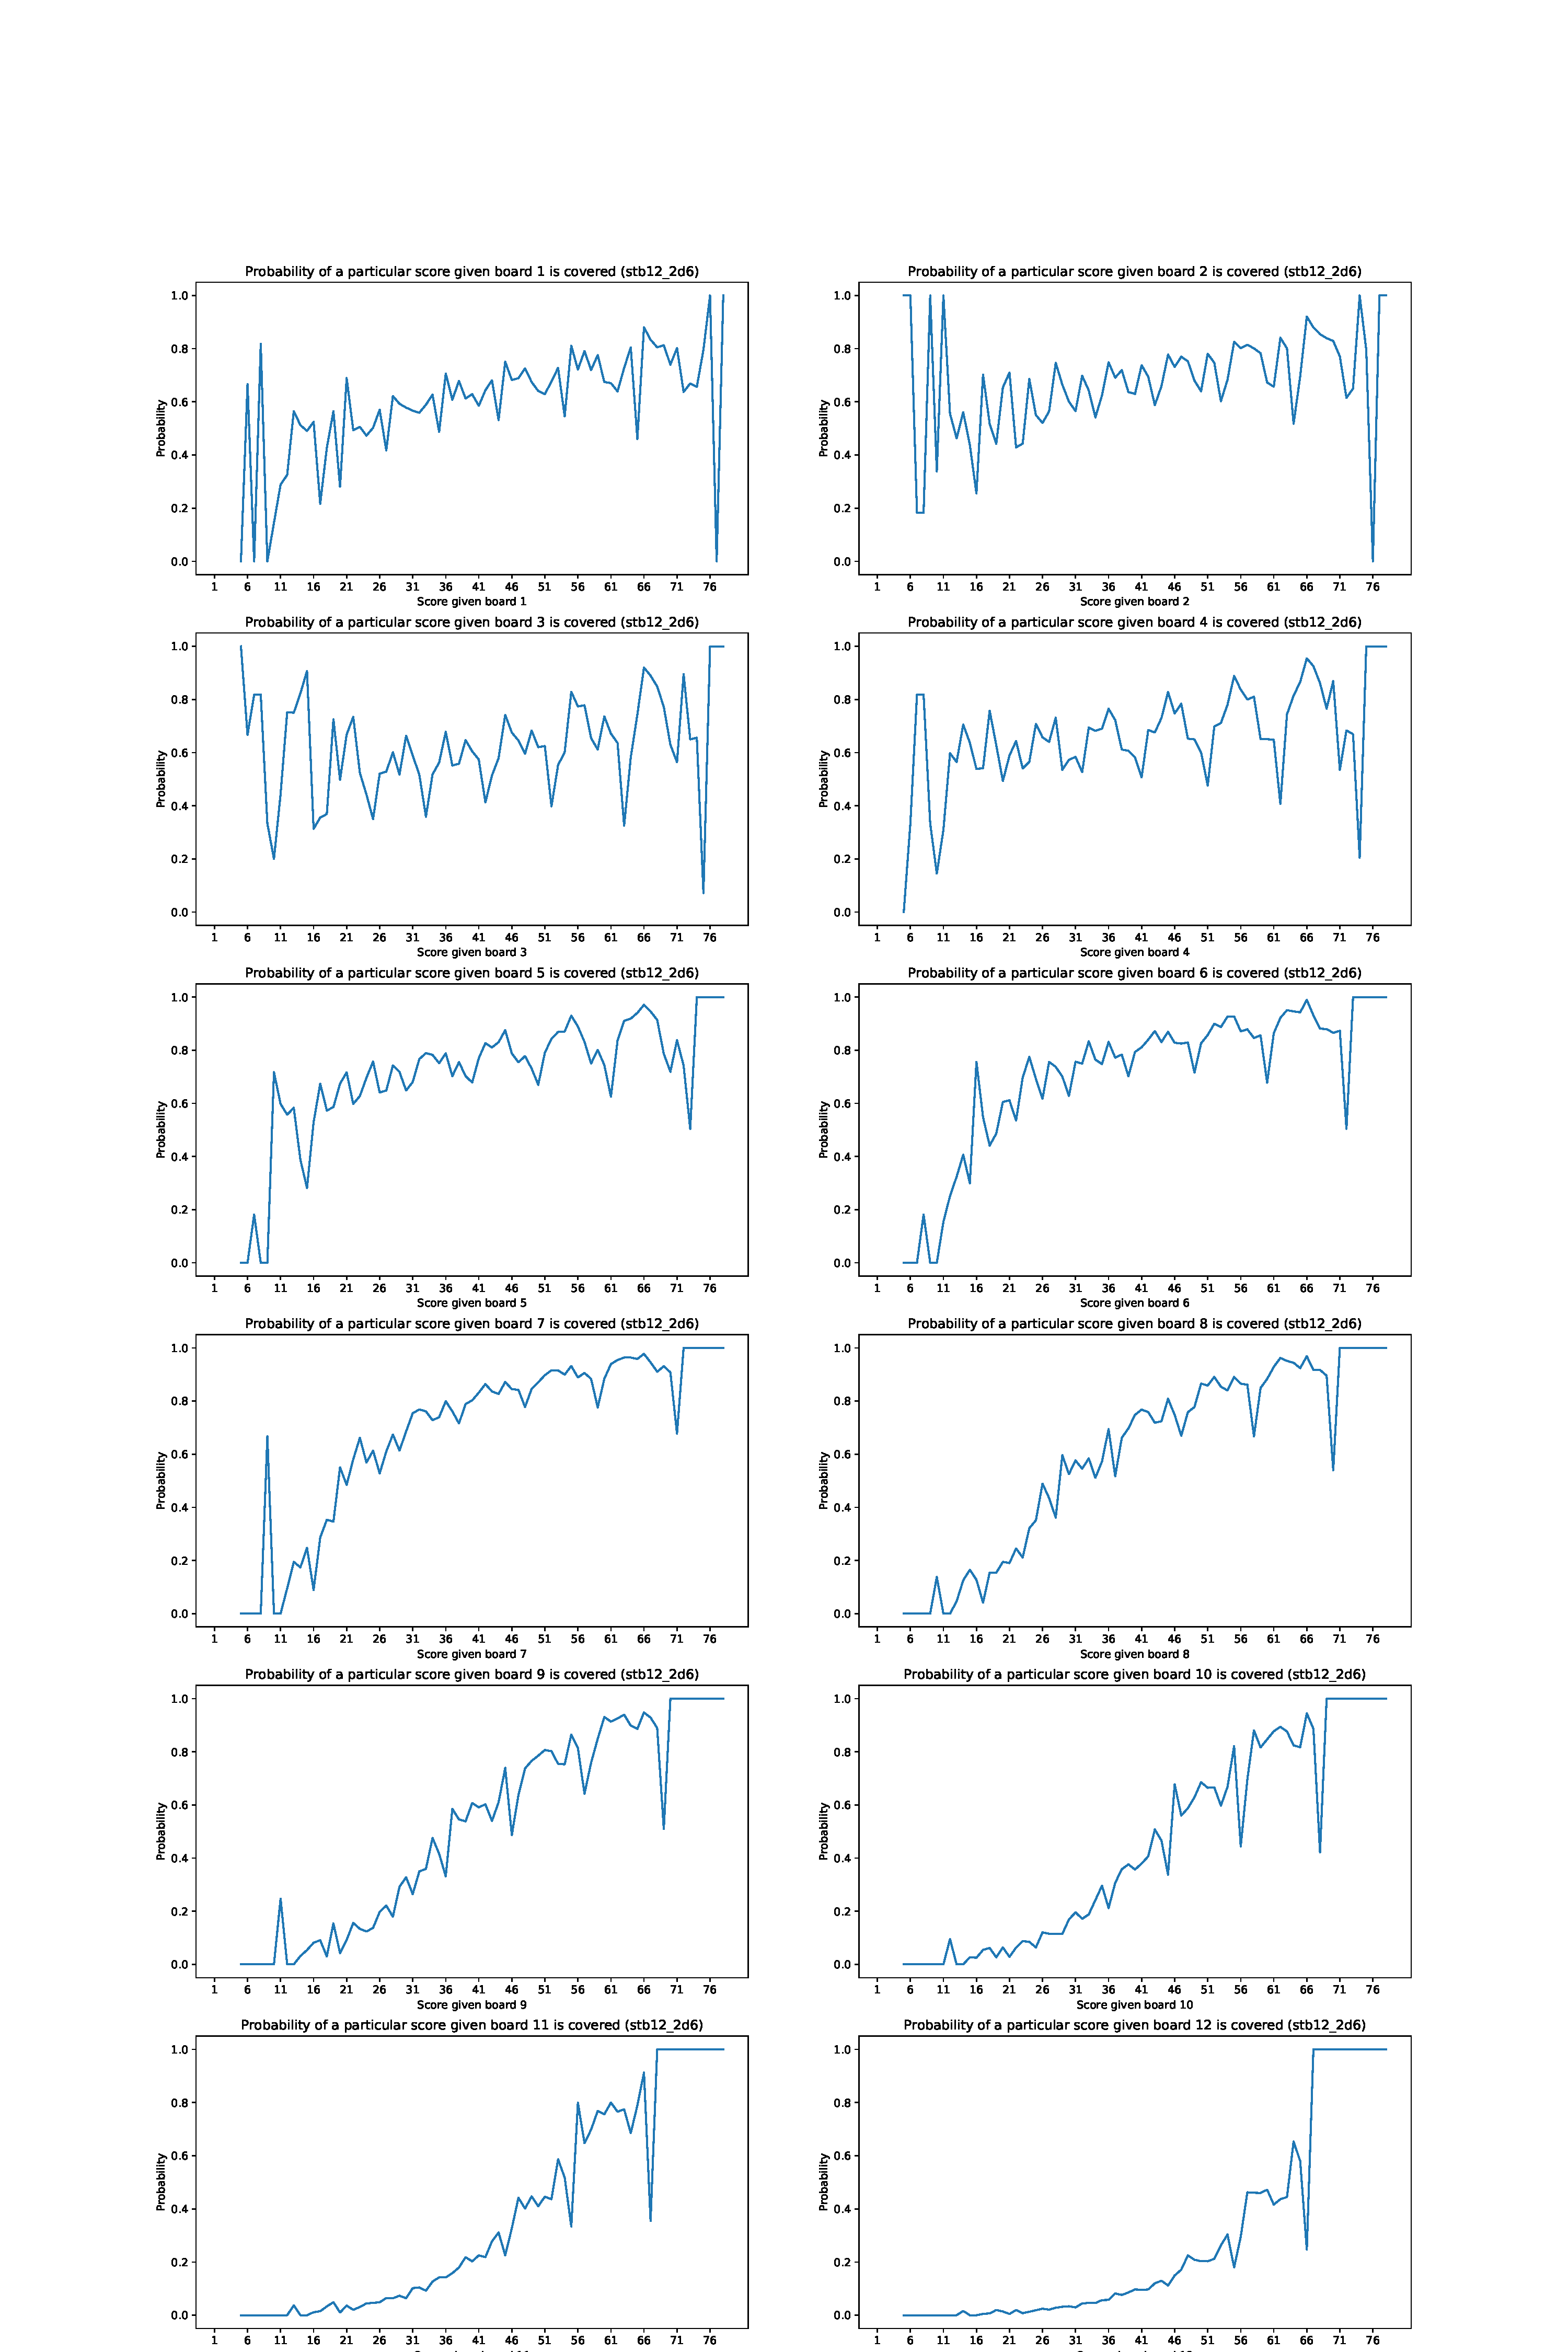
\includegraphics[width=\textwidth]{images/ShutTheBox/stb12_2d6_score_given_board_12.pdf}
    \caption{The conditional probability of each score in Shut the Box given board $n$ is covered, in the standard variant under the high-board strategy.}
\label{cs1:stb12_2d6_cond_prob}
\end{figure}

This idea can also be considered from a more combinatorial point of view. Given a dice roll of value $n$, each possible covering is a partition of $n$ into distinct parts, also known as a \emph{strict partition} of $n$. For instance, there are 27 possible coverings which cover board 1, but only 2 coverings which cover board 11, further exemplifying that opportunities to cover high boards are rare. This difference is exacerbated when multiple dice are used, including in the standard variant, since especially high dice rolls are rarer to obtain, compared to using one dice with a uniform probability of rolling each possible value.

\subsection{Comparing the optimal and high-board strategies}
\label{cs1:compare-strats}
Along with generating an optimal strategy, PRISM also provides support for exporting a graphical output of this optimal strategy, allowing potential comparisons between strategies. However, due to visualisation constraints, we only consider one variant of Shut the Box - the variant where 6 boards are used, and a single 6-sided die is rolled. While this variant is relatively small and simple, comparing the high-board strategy with the optimal strategy still leads to interesting behaviour. To exemplify this, consider the following example.

\begin{example}
\label{cs1:greedy-optimal}

Consider the strategy which maximises the expected score of Shut the Box, which is 21 for a 6-board variant. Now consider the situation presented in Figure \ref{cs1:optimal_high_board}, where boards 2, 4 and 6 are uncovered while a 6 is rolled. The optimal strategy chooses to cover boards 4 and 2, while the high-board strategy chooses to cover board 5 and 1.

\begin{figure}
    \centering
    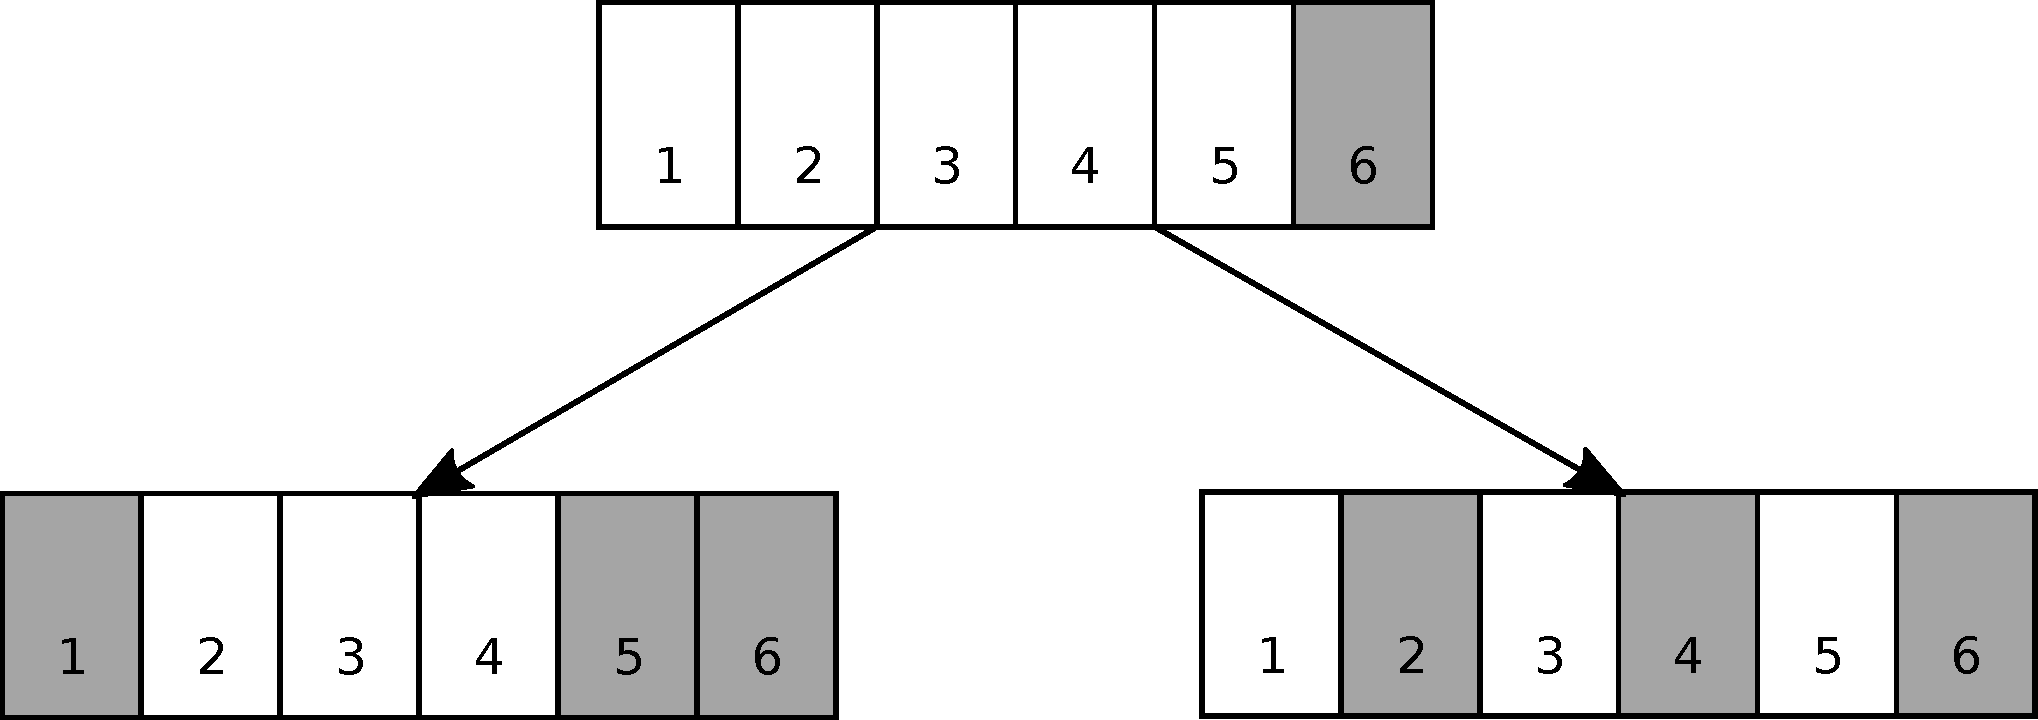
\includegraphics[width=\textwidth]{images/ShutTheBox/optimal_high_board.pdf}
    \caption{The optimal strategy covers boards 4 and 2, while the high-board strategy covers board 5 and 1. Covering boards 1, 2 and 3 is also possible, though neither strategy chooses this covering.}
\label{cs1:optimal_high_board}
\end{figure}

Two modified versions of the PRISM model of the 6-board variant of Shut the Box were created, with the nondeterministic model and the model under the high-board strategies modified to represent the decision made by each strategy respectively.

From this position, the expected score of the high-board strategy is 16.4167, while the expected score of the optimal strategy is 16.4230. This is unsurprising, since the optimal strategy is specifically generated to attain the maximum possible expected score.

However, the probability of attaining a perfect score is approximately 0.1389 under the highboard strategy, which is also the maximum possible probability of attaining a perfect score after covering boards 4 and 2. This suggests that the high board strategy is more likely to attain a perfect score, compared to the optimal strategy for attaining the maximum expected score, since a new optimal strategy is generated in order to calculate the maximum probability.

\end{example}

This presents an interesting trade-off between strategies - while the optimal strategy aims to maximise the expected score of Shut the Box (by design), the high-board strategy performs better when considering the probability of attaining the maximum possible score.

Inherently, this suggests the impact of risk in comparing different strategies. A trade-off exists between attaining a higher average score and attaining the maximum possible score, and this trade-off can be exploited in the design of Shut the Box.

For instance, suppose two players play a round of Shut the Box sequentially, aiming to get a higher score than the other player. The first player's aim is to get the highest score possible, but the second player's objective is simply to earn more points than the first player, regardless of the margin of victory. If the first player scores 20 points on the 6-board variant, the second player should play the aforementioned high-board strategy, since this has a higher probability of gaining 21 points, the only possible score which can win outright. On the other hand, if the first player scores very few points, then a more consistent strategy, such as the optimal expected score strategy, may be preferred, in order to maximise the probability of winning. Alternatively, an additional incentive could be provided to encourage players to attain a perfect score, such as a "jackpot" if Shut the Box is played as a gambling game.

\section{Evaluating the design of Shut the Box}


Overall, while we have shown the high-board strategy is successful (and conversely that the low-board strategy is unsuccessful), the results of Table \ref{cs1:exp_value_results} indicates the main flaw with Shut the Box. When designing games, optimal strategies should be sufficiently complex so that human players cannot feasibly recreate this strategy. Optimal strategies may be seen as less enjoyable for players to play with, since decisions at various points throughout a game are effectively defined beforehand, rather than the player making decisions and adapting during the game. 

While the optimal strategy for Shut the Box is somewhat complex, Section \ref{cs1:compare-strats} shows that a simple strategy is very close to optimal. This shows that Shut the Box is flawed, because the additional complexity involved in learning a more optimal strategy does not lead to a significant improvement in the overall outcome of the game. While the trade-off between risk and reward is potentially interesting, in most cases the difference is fairly small, so the impact of this trade-off is minimal. We have also suggested several possible variants of Shut the Box to alter the balance between risk and reward, such as the addition of a "jackpot" to emphasise riskier strategies, given the lack of differentiation between strategies these variants are unlikely to lead to meaningful changes in strategy.

Throughout this case study, we have introduced a perfect information game and compared manually created strategies to optimal strategies in order to evaluate the design of that game. Now we consider a different game, where the full state of the game is unknown to each player.